

\section{OpticalElement: \textquotedbl{}micado\_sci\_detector\textquotedbl{}%
  \label{opticalelement-micado-sci-detector}%
}

\textbf{Element}: detector

\textbf{Alias}: DET

\textbf{Description}: List of MICADO detector effects relevant for astronomers


\subsection{Global properties%
  \label{global-properties}%
}

\begin{quote}
\begin{alltt}
\begin{lstlisting}[frame=single]
image_plane_id : 0
   temperature : -230
           dit : !OBS.dit
          ndit : !OBS.ndit
         width : 4096
        height : 4096
  element_name : micado_sci_detector
\end{lstlisting}
\end{alltt}
\end{quote}


\subsection{Effects%
  \label{effects}%
}

Summary of Effects included in this optical element:

\setlength{\DUtablewidth}{\linewidth}
\begin{longtable*}[c]{|p{0.212\DUtablewidth}|p{0.170\DUtablewidth}|p{0.263\DUtablewidth}|p{0.098\DUtablewidth}|p{0.212\DUtablewidth}|}
\hline
\textbf{%
element
} & \textbf{%
name
} & \textbf{%
class
} & \textbf{%
included
} & \textbf{%
z\_orders
} \\
\hline
\endfirsthead
\hline
\textbf{%
element
} & \textbf{%
name
} & \textbf{%
class
} & \textbf{%
included
} & \textbf{%
z\_orders
} \\
\hline
\endhead
\multicolumn{5}{c}{\hfill ... continued on next page} \\
\endfoot
\endlastfoot

micado\_sci\_detector
 & 
detector\_window
 & 
DetectorWindow
 & 
True
 & 
{[}90, 290, 390, 490{]}
 \\
\hline

micado\_sci\_detector
 & 
qe\_curve
 & 
QuantumEfficiencyCurve
 & 
True
 & 
{[}113, 513{]}
 \\
\hline

micado\_sci\_detector
 & 
exposure\_action
 & 
SummedExposure
 & 
True
 & 
{[}860{]}
 \\
\hline

micado\_sci\_detector
 & 
dark\_current
 & 
DarkCurrent
 & 
True
 & 
{[}830{]}
 \\
\hline

micado\_sci\_detector
 & 
shot\_noise
 & 
ShotNoise
 & 
True
 & 
{[}820{]}
 \\
\hline

micado\_sci\_detector
 & 
readout\_noise
 & 
PoorMansHxRGReadoutNoise
 & 
True
 & 
{[}811{]}
 \\
\hline
\end{longtable*}
\label{tbl-micado-sci-detector}


\subsubsection{DetectorWindow: \textquotedbl{}detector\_window\textquotedbl{}%
  \label{detectorwindow-detector-window}%
}

\textbf{Included by default}: \texttt{True}

\textbf{File Description}:

\textbf{Class Description}: For when a full DetectorList if too cumbersome

\textbf{Changes}:

\begin{itemize}
\item \end{itemize}


\paragraph{Data%
  \label{data}%
}

\begin{figure}[H]
\noindent\makebox[\linewidth][c]{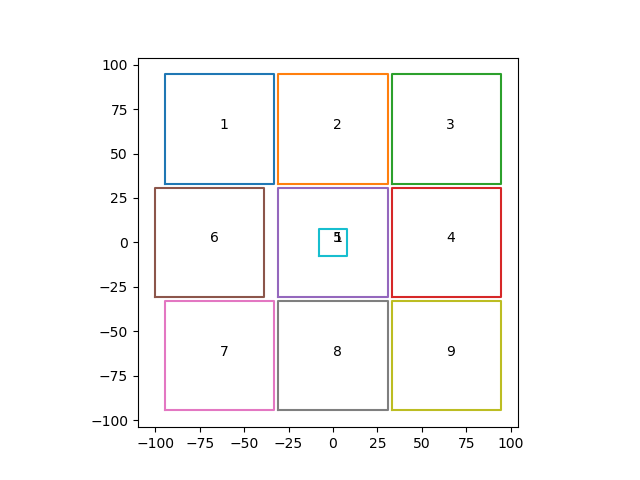
\includegraphics{detector_window.png}}\phantomsection\label{fig-detector-window}
\end{figure}

\setlength{\DUtablewidth}{\linewidth}
\begin{longtable*}[c]{|p{0.051\DUtablewidth}|p{0.075\DUtablewidth}|p{0.075\DUtablewidth}|p{0.133\DUtablewidth}|p{0.145\DUtablewidth}|p{0.075\DUtablewidth}|p{0.063\DUtablewidth}|p{0.133\DUtablewidth}|}
\hline
\textbf{%
id
} & \textbf{%
x\_cen
} & \textbf{%
y\_cen
} & \textbf{%
x\_size
} & \textbf{%
y\_size
} & \textbf{%
angle
} & \textbf{%
gain
} & \textbf{%
pixel\_size
} \\
\hline
\endfirsthead
\hline
\textbf{%
id
} & \textbf{%
x\_cen
} & \textbf{%
y\_cen
} & \textbf{%
x\_size
} & \textbf{%
y\_size
} & \textbf{%
angle
} & \textbf{%
gain
} & \textbf{%
pixel\_size
} \\
\hline
\endhead
\multicolumn{8}{c}{\hfill ... continued on next page} \\
\endfoot
\endlastfoot

0
 & 
0.0
 & 
0.0
 & 
!DET.width
 & 
!DET.height
 & 
0
 & 
1
 & 
0.015
 \\
\hline
\end{longtable*}
\label{tbl-detector-window}


\paragraph{Meta-data%
  \label{meta-data}%
}

\begin{quote}
\begin{alltt}
\begin{lstlisting}[frame=single]
       filename : None
           name : detector_window
     orig_units : pixel
     x_cen_unit : pixel
     y_cen_unit : pixel
    x_size_unit : pixel
    y_size_unit : pixel
pixel_size_unit : mm
     angle_unit : deg
      gain_unit : electron/adu
 image_plane_id : 0
    temperature : -230
            dit : !OBS.dit
           ndit : !OBS.ndit
   element_name : micado_sci_detector
        z_order : [90, 290, 390, 490]
        include : True
          table :  id x_cen y_cen   x_size      y_size   angle gain pixel_size
\end{lstlisting}
\end{alltt}
\end{quote}

\DUadmonition[system-message]{
\DUtitle[system-message]{system-message}


{\color{red}WARNING/2} in \texttt{<string>}, line~104

Literal block ends without a blank line; unexpected unindent.
backrefs: }

\begin{description}
\item[{-{}-{}- -{}-{}-{}-{}- -{}-{}-{}-{}- -{}-{}-{}-{}-{}-{}-{}-{}-{}- -{}-{}-{}-{}-{}-{}-{}-{}-{}-{}- -{}-{}-{}-{}- -{}-{}-{}- -{}-{}-{}-{}-{}-{}-{}-{}-{}-}] \leavevmode 
\begin{description}
\item[{0   0.0   0.0 !DET.width !DET.height     0    1      0.015}] \leavevmode 
\begin{quote}
\begin{quote}
\begin{quote}
pixel\_scale : !INST.pixel\_scale
\end{quote}

\DUadmonition[system-message]{
\DUtitle[system-message]{system-message}


{\color{red}WARNING/2} in \texttt{<string>}, line~107

Block quote ends without a blank line; unexpected unindent.
backrefs: }

active\_detectors : all
\end{quote}

\DUadmonition[system-message]{
\DUtitle[system-message]{system-message}


{\color{red}WARNING/2} in \texttt{<string>}, line~108

Block quote ends without a blank line; unexpected unindent.
backrefs: }

report\_plot\_include : True
\end{quote}

\DUadmonition[system-message]{
\DUtitle[system-message]{system-message}


{\color{red}WARNING/2} in \texttt{<string>}, line~109

Block quote ends without a blank line; unexpected unindent.
backrefs: }

report\_table\_include : True

\end{description}

\end{description}


\subsubsection{QuantumEfficiencyCurve: \textquotedbl{}qe\_curve\textquotedbl{}%
  \label{quantumefficiencycurve-qe-curve}%
}

\textbf{Included by default}: \texttt{True}

\textbf{File Description}: Quantum efficiency curves for each detector

\textbf{Class Description}: <no docstring>

\textbf{Changes}:

\begin{itemize}
\item \{datetime.date(2018, 11, 19): '(KL) updated meta data to new format'\}

\item \{datetime.date(2019, 8, 9): '(KL) Added action keyword to meta data'\}
\end{itemize}


\paragraph{Data%
  \label{id1}%
}


\paragraph{Meta-data%
  \label{id2}%
}

\begin{quote}
\begin{alltt}
\begin{lstlisting}[frame=single]
       filename : QE_detector_H2RG.dat
           name : qe_curve
 image_plane_id : 0
    temperature : -230
            dit : !OBS.dit
           ndit : !OBS.ndit
          width : 4096
         height : 4096
   element_name : micado_sci_detector
         author : Kieran Leschinski
        sources : Finger+ 2008 SPIE
   date_created : 2016-01-01
  date_modified : 2019-08-09
           type : detector:quantum_efficiency
         status : Design - guestimated by reading off the graph in Finger+ 2008
wavelength_unit : um
         action : transmission
        z_order : [113, 513]
        include : True
   ignore_wings : False
       wave_min : !SIM.spectral.wave_min
       wave_max : !SIM.spectral.wave_max
      wave_unit : !SIM.spectral.wave_unit
       wave_bin : !SIM.spectral.spectral_resolution
       position : -1
\end{lstlisting}
\end{alltt}
\end{quote}


\subsubsection{SummedExposure: \textquotedbl{}exposure\_action\textquotedbl{}%
  \label{summedexposure-exposure-action}%
}

\textbf{Included by default}: \texttt{True}

\textbf{File Description}: Summing up sky signal for all DITs and NDITs

\textbf{Class Description}: <no docstring>

\textbf{Changes}:

\begin{itemize}
\item \end{itemize}


\paragraph{Data%
  \label{id3}%
}


\paragraph{Meta-data%
  \label{id4}%
}

\begin{quote}
\begin{alltt}
\begin{lstlisting}[frame=single]
      filename : None
          name : exposure_action
image_plane_id : 0
   temperature : -230
           dit : !OBS.dit
          ndit : !OBS.ndit
         width : 4096
        height : 4096
  element_name : micado_sci_detector
       z_order : [860]
       include : True
\end{lstlisting}
\end{alltt}
\end{quote}


\subsubsection{DarkCurrent: \textquotedbl{}dark\_current\textquotedbl{}%
  \label{darkcurrent-dark-current}%
}

\textbf{Included by default}: \texttt{True}

\textbf{File Description}: MICADO dark current

\textbf{Class Description}: required: dit, ndit, value

\textbf{Changes}:

\begin{itemize}
\item \end{itemize}


\paragraph{Data%
  \label{id5}%
}


\paragraph{Meta-data%
  \label{id6}%
}

\begin{quote}
\begin{alltt}
\begin{lstlisting}[frame=single]
      filename : None
          name : dark_current
image_plane_id : 0
   temperature : -230
           dit : !OBS.dit
          ndit : !OBS.ndit
         width : 4096
        height : 4096
  element_name : micado_sci_detector
         value : 0.1
       z_order : [830]
       include : True
\end{lstlisting}
\end{alltt}
\end{quote}


\subsubsection{ShotNoise: \textquotedbl{}shot\_noise\textquotedbl{}%
  \label{shotnoise-shot-noise}%
}

\textbf{Included by default}: \texttt{True}

\textbf{File Description}: apply poisson shot noise to images

\textbf{Class Description}: <no docstring>

\textbf{Changes}:

\begin{itemize}
\item \end{itemize}


\paragraph{Data%
  \label{id7}%
}


\paragraph{Meta-data%
  \label{id8}%
}

\begin{quote}
\begin{alltt}
\begin{lstlisting}[frame=single]
      filename : None
          name : shot_noise
image_plane_id : 0
   temperature : -230
           dit : !OBS.dit
          ndit : !OBS.ndit
         width : 4096
        height : 4096
  element_name : micado_sci_detector
       z_order : [820]
       include : True
   random_seed : !SIM.random.seed
\end{lstlisting}
\end{alltt}
\end{quote}


\subsubsection{PoorMansHxRGReadoutNoise: \textquotedbl{}readout\_noise\textquotedbl{}%
  \label{poormanshxrgreadoutnoise-readout-noise}%
}

\textbf{Included by default}: \texttt{True}

\textbf{File Description}: Readout noise frames

\textbf{Class Description}: <no docstring>

\textbf{Changes}:

\begin{itemize}
\item \end{itemize}


\paragraph{Data%
  \label{id9}%
}


\paragraph{Meta-data%
  \label{id10}%
}

\begin{quote}
\begin{alltt}
\begin{lstlisting}[frame=single]
         filename : None
             name : readout_noise
   image_plane_id : 0
      temperature : -230
              dit : !OBS.dit
             ndit : !OBS.ndit
            width : 4096
           height : 4096
     element_name : micado_sci_detector
        noise_std : 12
       n_channels : 64
          z_order : [811]
          include : True
pedestal_fraction : 0.3
    read_fraction : 0.4
    line_fraction : 0.25
 channel_fraction : 0.05
      random_seed : !SIM.random.seed
\end{lstlisting}
\end{alltt}
\end{quote}
